This section is solely present to guide the reader to other sources where help can be obtained in case something goes wrong. This manul strives to describe many possible scenarios, however when it comes to troubleshooting, it is best to consult these sources. 

\section{Ubuntu Help}
Getting help to troubleshoot Ubuntu is very easy due to the active community behind it. You are not limited to getting help from the company behind Ubuntu itself but rather the entire Ubuntu community which consist of millions of users. There are forums, IRC chat rooms and official Ubuntu documentation out there to help you. You can get an answer to your  question within minutes at these websites since they are run by the community. You can also get help in your own local languages if you are not comfortable with English. The most popular sources are described below.

\subsection*{Official Ubuntu documentation}
This is the official Ubuntu documentation provided by Ubuntu. Here you can find instructions to installing packages, using Ubuntu and pretty much everything. It is the holy grail of Ubuntu documentation. You can find their website at \href{https://help.ubuntu.com/}{https://help.ubuntu.com/}.

\begin{figure}[h!]	
	\centering
	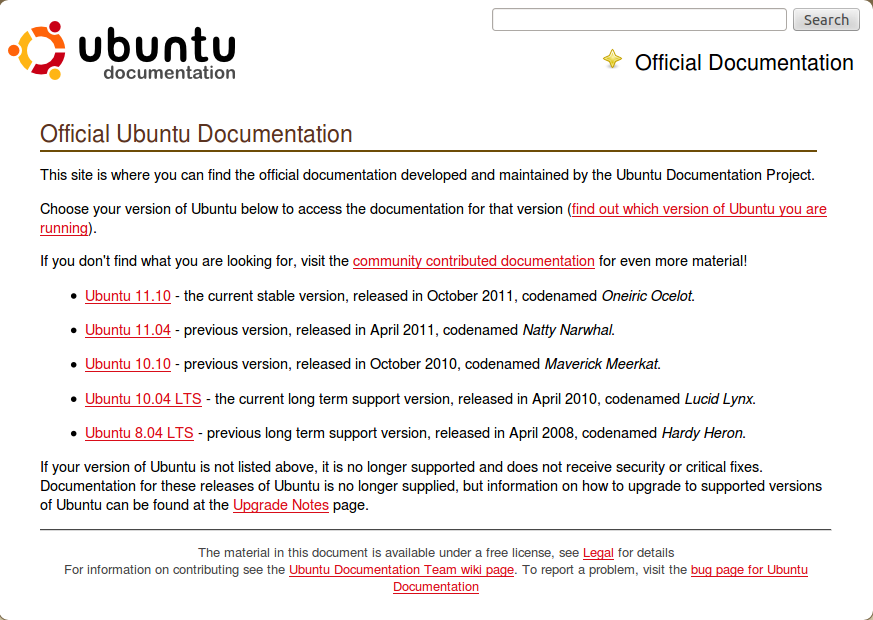
\includegraphics[width=350pt]{./images/get-help/officialubuntuhelp.png}
	\caption{Official Ubuntu Documentation}	
	\label{fig:official-ubuntu-help}		
\end{figure}

\subsection*{Ubuntu Forums} \index{Help} \index{Forums}
As the name suggestions, this is the official Ubuntu forum where you can ask queries, and get help to troubleshoot any problems you might face. The queries can be related to anything about Ubuntu. It could be a specific problem that you alone face and you will still find answers to them here. This forum is more personal and by directly enquiring about your problem, there is a good chance that you will be able to solve your problem quicker. This is also a place to discuss your issues. You can find the website at \href{http://ubuntuforums.org/}{http://ubuntuforums.org/}.

\begin{figure}[h!]	
	\centering
	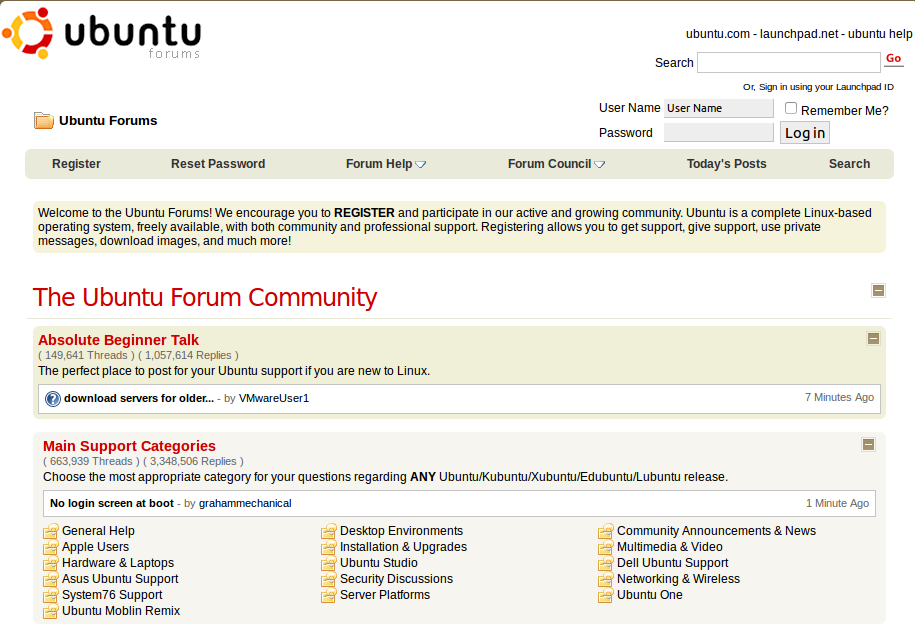
\includegraphics[width=350pt]{./images/get-help/ubuntuforums.png}
	\caption{Official Ubuntu Forums}	
	\label{fig:ubuntuforums}		
\end{figure}

\subsection*{AskUbuntu}
AskUbuntu is a community driven Q\&A for Ubuntu users. In this website, the questions raised are specific and short. How is this different from Ubuntu forums? Well, in AskUbuntu you have a question raised by a user which is followed by several answers by the community. These answers can be voted upon, and the most popular answer (the most correct one) rises to the top giving you a exact answer to your question. Open-ended questions like your opinion of Ubuntu etc, are generally not welcome in this website. You can access the website at \href{http://askubuntu.com/}{http://askubuntu.com/}.

\begin{figure}[h!]	
	\centering
	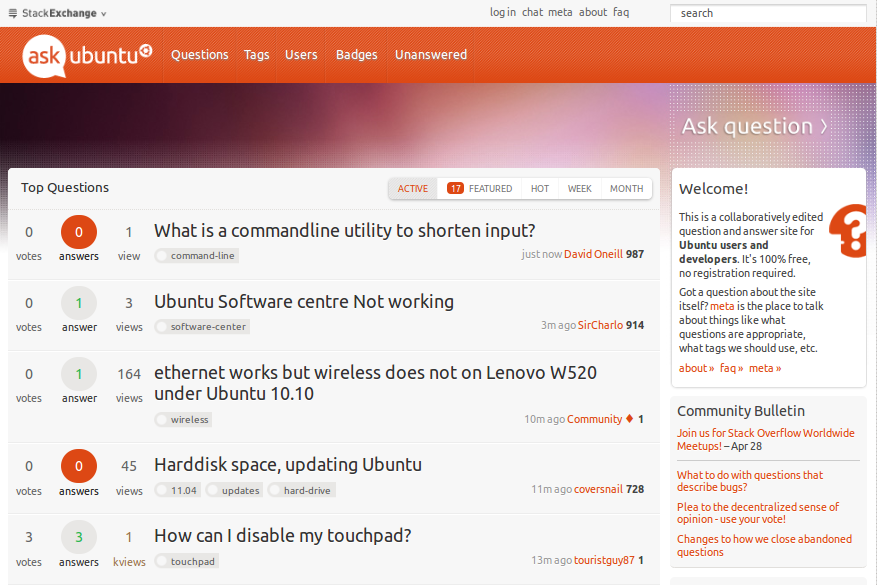
\includegraphics[width=350pt]{./images/get-help/askubuntu.png}
	\caption{AskUbuntu}	
	\label{fig:askubuntu}		
\end{figure}

\subsection*{Local Community} \index{Local Community}
If you come from a country where English is not natively spoken there is a good chance that there is a  local Ubuntu web sites and a community website. You can find more information about the local community teams at \href{https://wiki.ubuntu.com/LoCoTeams}{https://wiki.ubuntu.com/LoCoTeams}. Since these teams are local, you can join them in their meetings and they will help you directly. In fact this is strongly recommended if you run into problems since directly meeting people who speak your language and know Ubuntu well are the easiest and quickest ways of solving issues.

\begin{figure}[h!]	
	\centering
	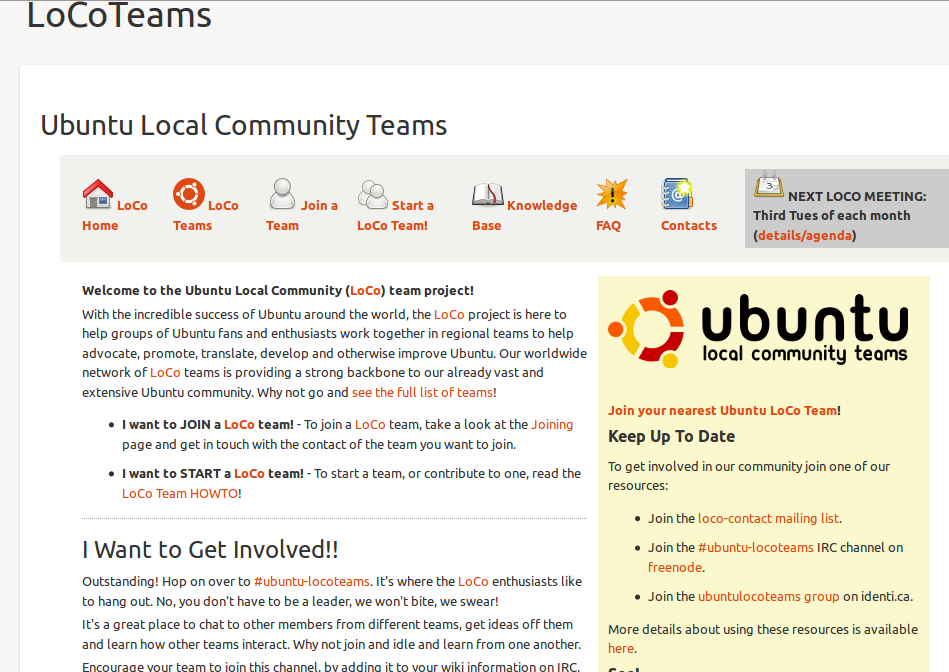
\includegraphics[width=350pt]{./images/get-help/locoteams.png}
	\caption{Ubuntu Local Community Teams}	
	\label{fig:locoteams}		
\end{figure}

\section{Latest news in the Ubuntu world} \index{News}
If you are interested to keep up to date with the latest news in the Ubuntu world there are many websites out there doing just this. Some reliable sources of news feed about the latest in the Ubuntu world are mentioned. Some of them are maintained by the company behind Ubuntu. This way you can be sure that they are reliable sources of information. There are also a sea of blogs/web sites/people talking/writing about Ubuntu. But not all of them are current.  Web sites that have the most current content about Ubuntu are: 

\begin{itemize}
\item \href{http://www.ubuntu.com}{Ubuntu} - The official Ubuntu website
\item \href{http://design.canonical.com/}{Canonical} - This is highly recommended since it provides information about new designs which will part of future releases of Ubuntu.
\item \href{http://markshuttleworth.com/}{Mark Shuttleworth Blog} - Blog maintained by Mark Shuttleworth, the founder of Ubuntu
\item \href{http://www.muktware.com/}{Muktware} - Website with the current news about open source technology such as Linux, Ubuntu, and other open source related news.
\item \href{http://www.omgubuntu.co.uk/}{OMG!Ubuntu} - Website Blog providing daily news about Ubuntu
\end{itemize}

\par \noindent It is also recommended to read news related to Ubuntu via social networks like Facebook, Google+, Twitter etc. This way might be the easiest way to stay in touch with the latest news not only related to Ubuntu but technology in general.
